\section{Issues of Cyclic Pursuit}

The formulation we have just described has two main issues:
\begin{itemize}
	\item The stability of the algorithm relies completely on geometrical criteria on the circle. These criteria are independent of the radius implying there is no control on the radius nor stability under perturbations.
	
	\item The convergence of the algorithm to a circle relies on achieving the $\alpha \mathbb{1} = \pi$ criterion. This implies the need of coordination and that if an agent leaves or joins the formation it will typically become unstable. We call this the resilience issue.
\end{itemize}

We will work on these two issues. A solution to the second one is provided in \cite{ramirez2010distributed}. This solution however, is dependent on the $\alpha \mathbb{1} = \pi$ condition and therefore is not considered to be resilient enough. In order to provide a better understanding of the solution we will first give a more insightful description of the two issues that will be addressed in this project.

\subsection{Radius stability}

While we have stated the conditions for convergence of the formation to a circle these conditions are only dependent on angles and phase constraints. This means that the radius of the formation is not involved in anyway so there is no control nor stability of the radius of the formation.
\\

One example of perturbations would be the wind blowing on formation or orbital decay. Errors can be simulated easily by decreasing the precision of the numerical integration. The solution displayed in the Problem formulation was obtained using MATLAB's ode45 solver. If we use Euler's method the solver accuracy decreases and incrementing the simulation time we can observe the effect of the numerical integration on the formation

\begin{figure}[H]
	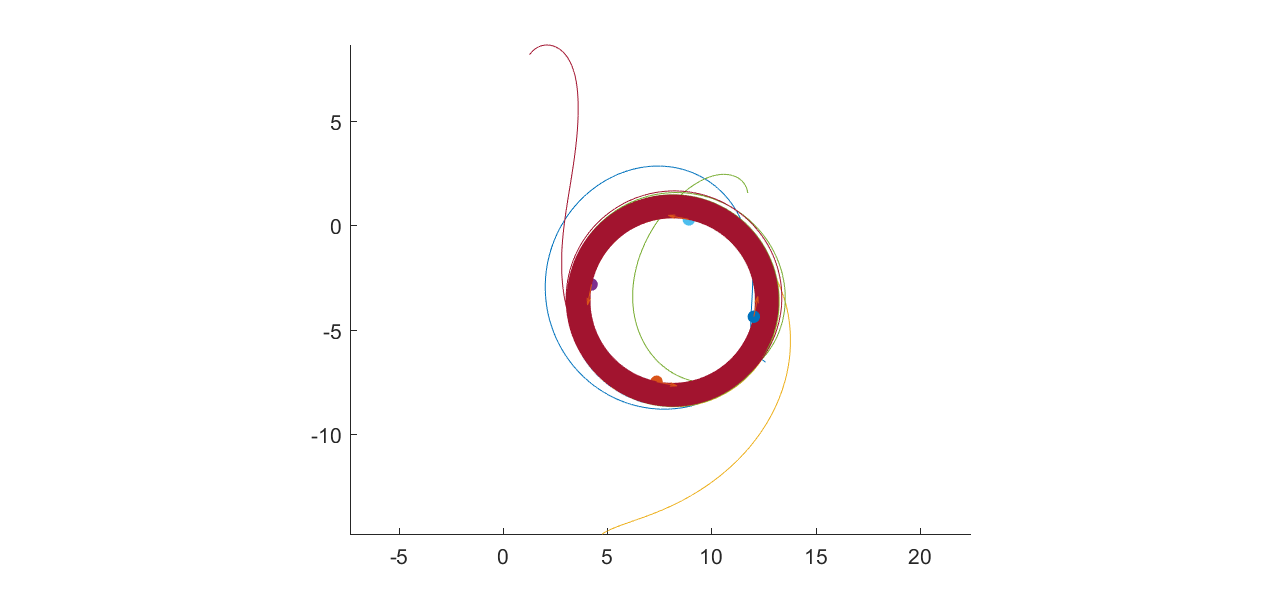
\includegraphics[width=\linewidth]{Attachments/Figure31.png}
	\caption{Formation Decay}
	\label{fig:Decay}
\end{figure}

The decay of the trajectory can be noticed by the thickness of the ring of trajectories, meaning they are decaying continuously.

Another issue is the difficulty to predict the parameters of the final formation given the initial conditions. We can check that if we swap the initial conditions for two agents the final radius and center of the formation change significantly, meaning it is not possible to predict the behavior of the system. Take as example the following simulation where the blue and yellow trajectories are interchanged

\begin{figure}[H]
	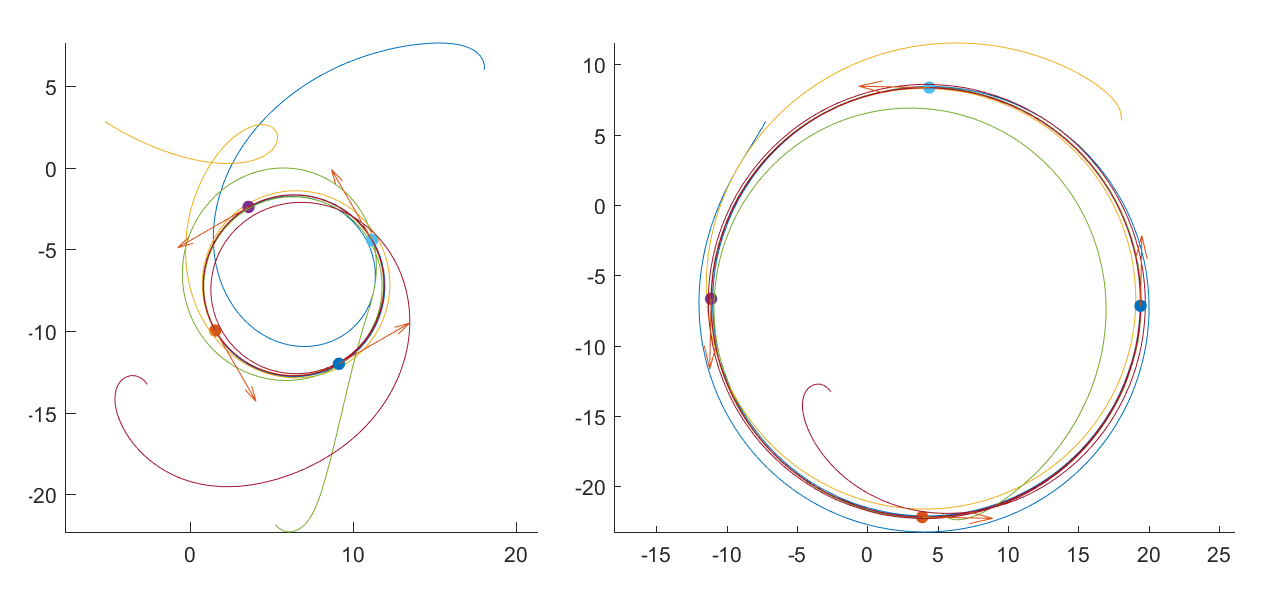
\includegraphics[width=\linewidth]{Attachments/Figure32.png}
	\caption{Swap of initial positions}
	\label{fig:Swap}
\end{figure}

Therefore a goal for the project is to modify the control law such that a predetermined specific formation radius can be achieved globally. This would imply that a stable and predictable formation can be achieved just based on the control law and references.

\subsection{Network dependence}
As it was described in the problem formulation, in order for the system to converge into a circle the $\alpha^*$ vector must satisfy certain conditions. These conditions are network dependent on the size of agent network. Typically, adding a new agent will increase the sum of the elements of $\alpha^{*T} \mathbb{1}$ and removing an agent will reduce it.
\\

Let us say that the formation achieved in the problem introduction loses an agent without modifying the control law, then $\alpha^{*T} \mathbb{1}<\pi$ and the behavior of the formation would be
\begin{figure}[H]
	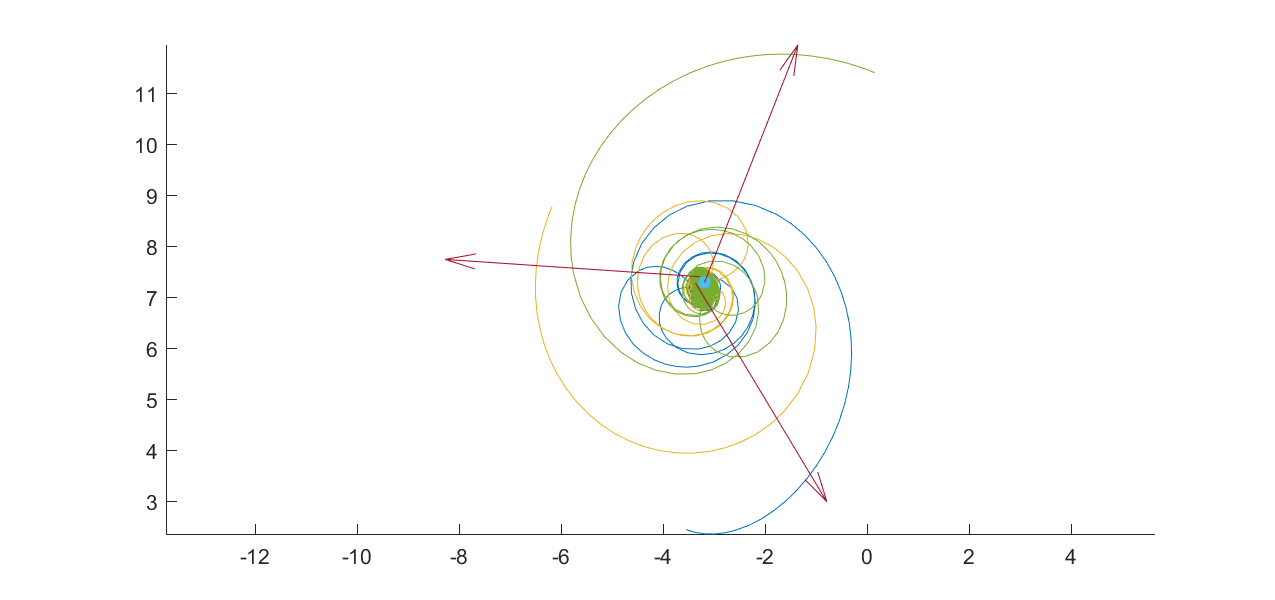
\includegraphics[width=\linewidth]{Attachments/Figure33.png}
	\caption{Formation collapse because of network change}
	\label{fig:Collapse}
\end{figure}

Yet again, we will try to overcome this issue by modifying the control law in a way that it adapts to the size of the network.
